\chapter{Intelligenztests}
Mit Hilfe von Intelligenztests soll ein Wert für den Generalfaktor g ermittelt werden, der es ermöglicht Personen miteinander zu vergleichen.

\section{Einsatzgebiete}
% Basis für wissenschaftliche Psychologie
% Schule / Bildung
% Auswahl Bewerber für Beruf
% Behandlung von Demenz
Es gibt viele verschiedene Intelligenztests, die für sehr unterschiedliche Anwendungen gedacht sind.

\paragraph{Basis für wissenschaftliche Psychologie}
Intelligenztests ermöglichen oft erst weitere Forschungen im Rahmen einer psychologischen Studie. So war auch die Entdeckung des Generalfaktors der Intelligenz erst durch die Analyse von Testergebnissen möglich.

\paragraph{Intelligenztests in Schule und Bildung}
Auch in der Schule spielen Intelligenztests eine wichtige Rolle, vor allem in den ersten Klassen. Bei auffälligen Kindern wird z. B. ein Intelligenztest durchegführt, um herauszufinden, ob diese die Schule wechseln sollten oder eine Klasse überspringen sollten. Diese Intelligenztests sind speziell auf das Alter der Kinder abgestimmt.

\paragraph{Mitarbeiterauswahl}
Bei manchen Stellenausschreibungen ist es erforderlich, dass die Bewerber einen Intelligenztest machen. Vor allem bei Stellen mit einer Vielzahl an Bewerbern kann dies genutzt werden, um einfach eine handvoll Bewerber auszuwählen.

\paragraph{Diagnose und Untersuchung von Demenz}
Umfangreiche Intelligenztests werden eingesetzt, um eine Demenzerkrankung zu diagnostizieren. Bei der Behandlung werden oft Schnelltests durchgeführt, die etwa 5 bis 10 Minuten dauern, um den Zustand des Patienten einzuschätzen und eventuell die Behandlung anzupassen.

\section{Binet-Simon-Skala}
Als erster \glqq seriöser\grqq{} Intelligenztest kann die Binet-Simon-Skala angesehen werden. Sie wurde vom französischen Bildungsministerium in Auftrag gegeben um eine objektive Einteilung von Kindern auf eine Sonderschule zu ermöglichen. Zuvor erfolgte dies durch eine Einschätzung des Lehrers, was oft zu Problemen geführt hat. Entwickelt wurde dieser Intelligenztest von den Franzosen Alfred Binet und Théodore Simon im Jahr 1905.

\paragraph{Aufbau}
Der Test besteht aus vielen Einzelaufgaben, die je nach Schwierigkeit in Altersklassen eingeteilt sind. Ein normal entwickeltes Kind aus diesen Alters sollte die Aufgabe lösen können. Einige Beispiele für diese Aufgaben sind:
\begin{itemize}
  \item{Das Unterscheiden von Rechts und Links}
  \item{Von 20 bis 0 rückwärts zählen}
  \item{Die Wörter eines Satzes in die richtige Reihenfolge bringen}
\end{itemize}

\paragraph{Auswertung}
Die höchste Altersklasse, aus der alle Aufgaben gelöst wurden, ist das Grundalter des Probanden.
Danach alle richtigen Aufgaben aus höheren Altersklasse als Anteile addiert. Dabei ist es egal, aus welcher höheren Altersklasse die Aufgabe gelöst wurde. Eine richtige Aufgabe aus dem Bereich 8 Jahre zählt genau so viel, wie eine richtige Aufgabe aus dem Bereich 10 Jahre.

Ein Kind hat zum Beispiel folgendes Ergebnis:

\begin{tabular}{l|lll}
  \textbf{Alter} & \textbf{Aufg. 1} & \textbf{Aufg. 2} & \textbf{Aufg. 3} \\
  3              & \cmark           & \cmark           & \cmark           \\
  4              & \cmark           & \cmark           & \cmark           \\
  5              & \xmark           & \cmark           & \xmark           \\
  6              & \xmark           & \xmark           & \cmark           \\
  7              & \xmark           & \xmark           & \xmark           \\
  8              & \xmark           & \xmark           & \xmark           \\
\end{tabular}

Sein geistiges Grundalter beträgt 4 Jahre, da es aus dieser Altersgruppe alle Aufgaben gelöst hat und in allen höheren Altersgruppen mindestens einen Fehler hat. Außerdem sind aus den höheren Altersgruppen noch 4 Aufgaben gelöst worden. Da es pro Gruppe von einem Jahr 3 Aufgaben gibt zählt eine Aufgabe:
$$ \frac{12\,\mathrm{Monate}}{3\,\mathrm{Aufgaben}} = 4\,\mathrm{Monate} $$
Diese Monatsanteile werden dann zum Grundalter addiert:
$$ 4\,\mathrm{Jahre} + 2 \times 4\,\mathrm{Monate} = 4\,\mathrm{Jahre}, 8\,\mathrm{Monate} $$
Dieses ermittelte geistige Alter wird dann mit dem tatsächlichen Lebensalter verglichen.
Wäre das getestete Kind z.B. 4 Jahre alt, dann wäre es überdurchschnittlich weit entwickelt. Würden die Ergebnisse aber
von einem 6-jährigen stammen, währe das Kind in seiner geistigen Entwicklung zurückgeblieben.

\paragraph{Vor- und Nachteile}
Die Binet-Simon-Skala war ein Durchbruch im Vergleich zu vorherigen Methoden. Sie findet (in abgewandelter Form) auch heute noch, über 100 Jahre später, Verwendung in Intelligenztests. In der beschriebenen ursprünglichen Variante hatte sie allerdings einige Probleme. Das größte Problem war, dass der reine Altersunterschied keine vergleichbaren Aussagen ermöglicht. Denn die Entwicklung eines Kindes verläuft nicht gleichmäßig. Kleinkinder entwickeln sich schneller als größere Kinder von z. B. 12 Jahren. Wenn also ein 5-jähriges Kind ein geistiges Alter von 4 Jahren hat, ist dies schlimmer als wenn ein 11-jähriges Kind ein geistiges Alter von 10 Jahren hat, obwohl der Altersunterschied in beiden Fällen 1 Jahr beträgt.

\section{Intelligenzquotient nach William Stern}
Aus dem Problem der Binet-Simon-Skala entwickelte William Stern den Intelligenzquotienten, der die Differenz zwischen Lebensalter und geistigem Alter vergleichbar machte. Dazu bildet er den Quotient aus Lebensalter und geistigem Alter.
$$ \mathrm{IQ} = \frac{\mathrm{Intelligenzalter}}{\mathrm{Lebensalter}} \times 100 $$
Der Quotient wird noch mit 100 multipliziert, um eine einfacher zu handhabende Zahl zu erhalten.

Wenn das Kind aus dem obigen Beispiel 4 Jahre alt, dann währe sein Intelligenzquotient

$$ \frac{4,667\,\mathrm{Jahre}}{4\,\mathrm{Jahre}} \times 100 \approx 117 $$
%TODO: Unify terms "geistiges Alter" and "Intelligenzalter"

\section{Intelligenzquotient heute}
Aber auch der Intelligenzquotient nach William Stern hatte ein Problem, was die Vergleichbarkeit der Werte angeht: Erwachsene Menschen entwickeln sich geistig nicht wirklich weiter. Zwischen einem 25-jährigen und einem 30-jährigen besteht kein Unterschied in der geistigen Entwicklung. Trotzdem haben sie bei gleichen Testergebnissen einen Unterschied im IQ von 20 Punkten.
$$ \frac{30}{30} \times 100 = 100 $$
$$ \frac{30}{25} \times 100 = 120 $$

Bei modernen Intelligenztest wird deshalb anders vorgegangen. Der Test wird mir einer Kontrollgruppe durchgeführt. Diese Kontrollgruppe ist je nach Test unterschiedlich aufgestellt. Alle gesellschaftlichen Gruppen sollten in ihr gleichmäßig vertreten sein (Geschlecht, Herkunft, Sozialer Status, etc.). Jedes Alter oder jede Altersgruppe erhält eine eigene Kontrollgruppe. Die Ergebnisse der Kontrollgruppe werden dann ausgewertet. Das Durchschnittliche Testergebnis der Kontrollgruppe entspricht einem IQ von 100.

\begin{figure}[H]
  \centering
  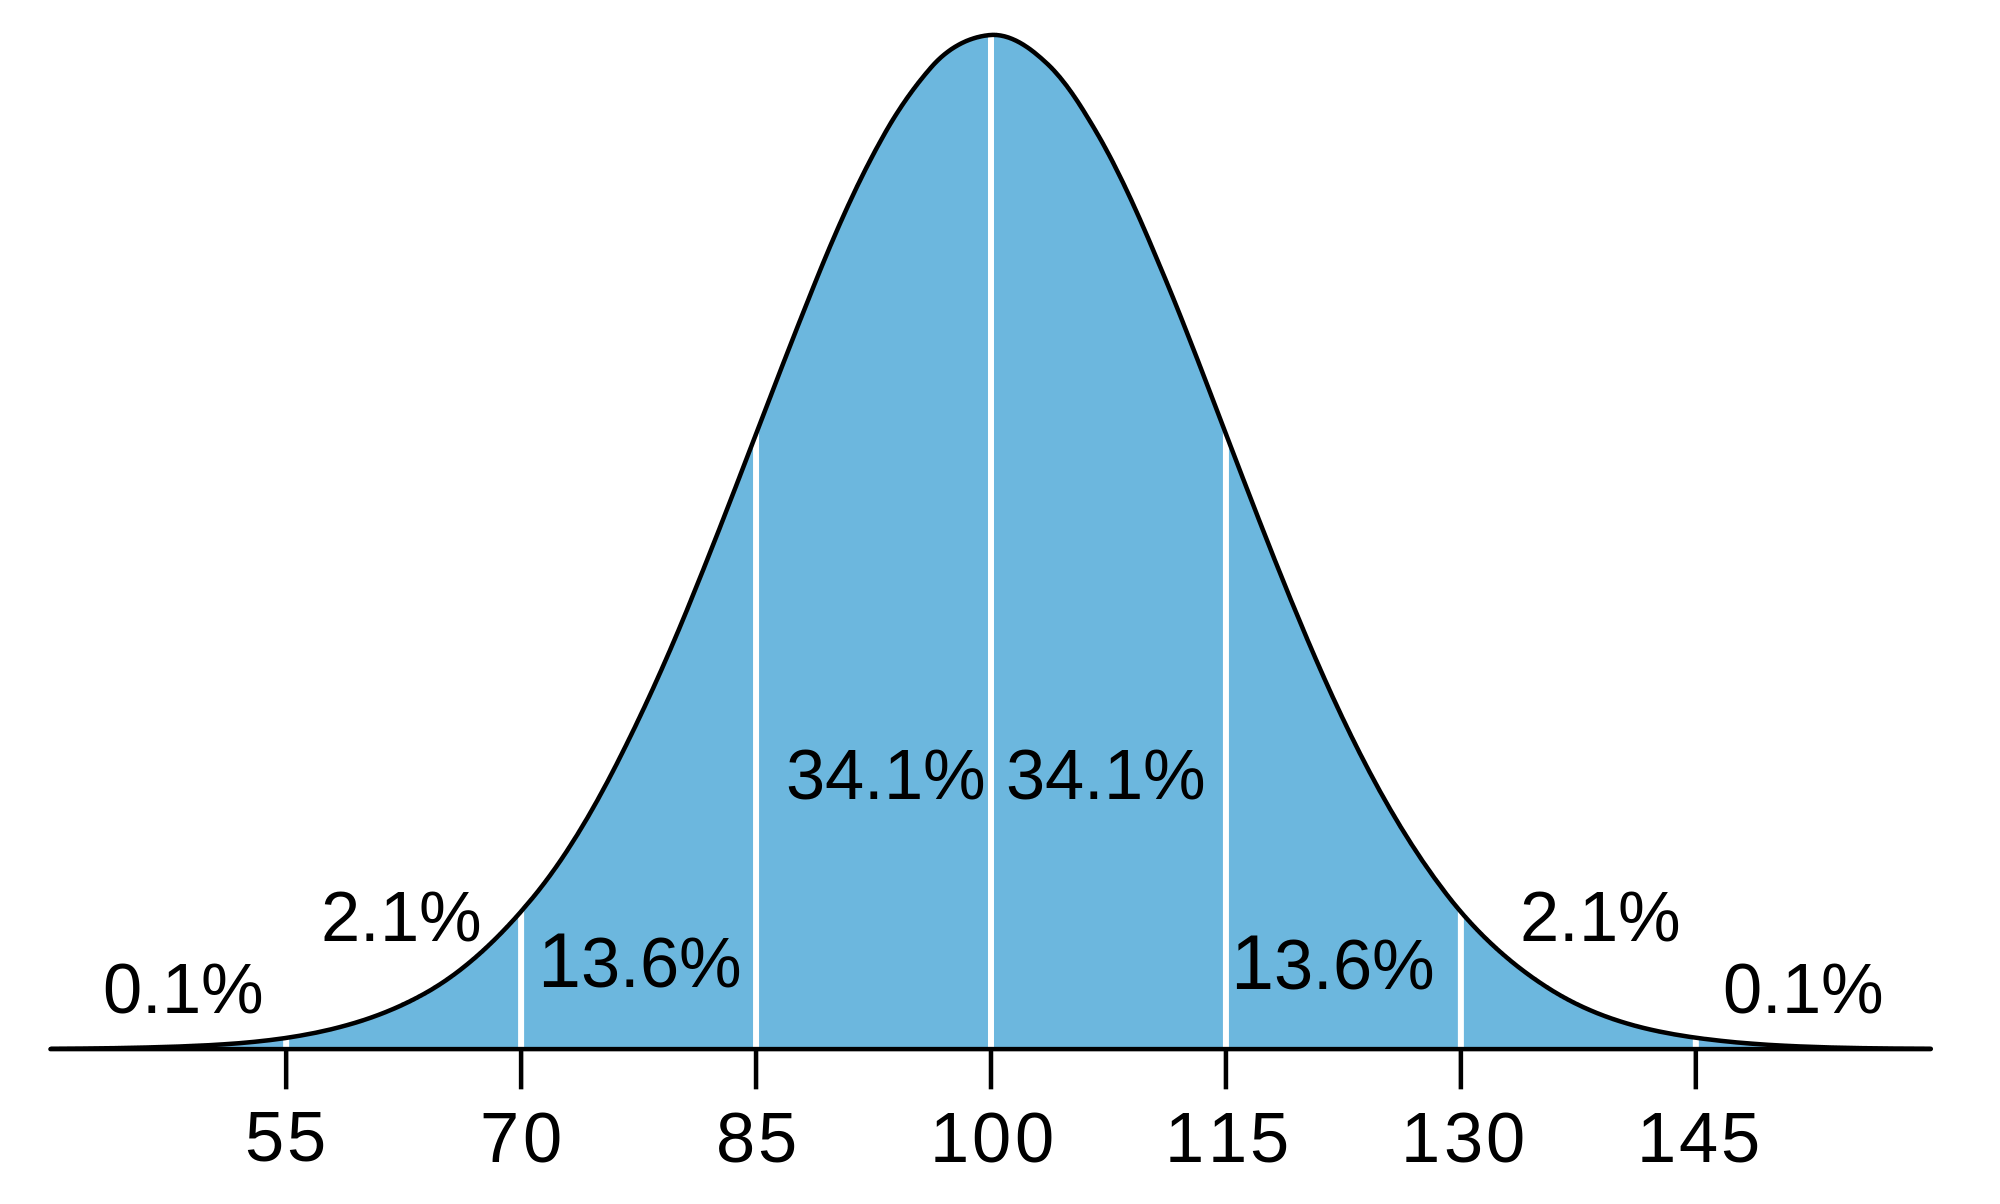
\includegraphics[width=0.6\textwidth]{img/IQ_distribution.png}
  \caption{Gewichtung des IQ \cite{wiki_img_iq}}
  \label{fig:iq}
\end{figure}

Die restlichen Testergebnisse werden nach einer bestimmten \emph{Standardverteilung} eingeordnet, so dass die Ergebnisse der Kontrollgruppe wie in Abb. \ref{fig:iq} verteilt sind.

\section{Der Flynn-Effekt}
\label{sec:flynn}

Der Flynn-Effekt wurde in den 1980er Jahren von James R. Flynn, einem amerikanischen Politikwissenschaftler, entdeckt. Er hat beobachtet, dass die durchschnittlichen IQ-Werte in den vergangenen Jahrzehnten merklich angestiegen sind.

Intelligenztests werden mit einer Kontrollgruppe durchgeführt und nach deren Ergebnissen werden die Probanden bewertet. Die letztendlichen Zahlenwerte haben sich also nicht verändert. Würde man aber heute einen Test durchführen und ihn mit den Ergebnissen einer Kontrollgruppe von 1950 vergleichen, dann Läge der durchschnittliche IQ der heutigen Teilnehmer bei 120.

\begin{figure}[H]
  \centering
  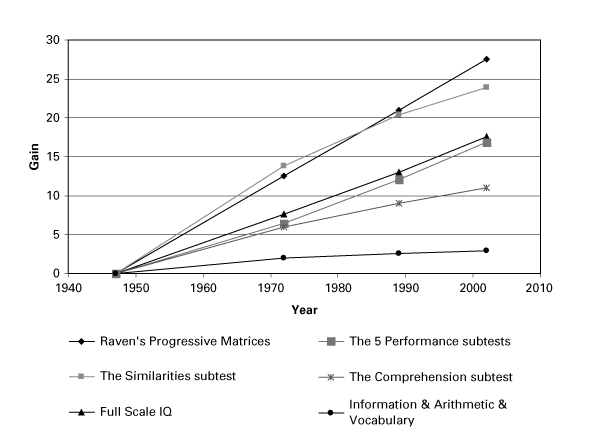
\includegraphics[width=0.6\textwidth]{img/Flynn.png}
  \caption{Entwicklung des IQ in den USA von 1947 bis 2002 \cite{flynn}}
  \label{fig:flynn}
\end{figure}

Umgekehrt, läge der Durchschnitts-IQ 1950 aus heutiger Sicht bei 70, die Grenze zu \glqq Geistiger Zurückgebliebenheit\grqq{}
\cite{ted_flynn}

Einen solch drastischen IQ-Unterschied müsste man im Verhalten bemerken können. Flynn und andere Wissenschaftler folgern aus dieser Entdeckung, das Intelligenztests nicht allein die Intelligenz messen, sondern nur die Fähigkeit, Tests zu bestehen.

Ein weiteres Indiz dafür ist, dass die größten Zunahmen in Logik-Tests zu beobachten sind, wie zum Beispiel ganz deutlich in \glqq Raven's Progressiven Matrizen \grqq{} festzustellen. Bei diesem Test geht es darum, eine Reihe von geometrischen Bildern zu ergänzen (siehe Abb. \ref{fig:ravens}).

\begin{figure}[H]
  \centering
  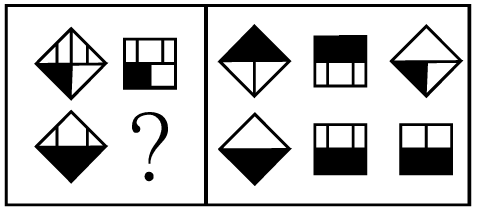
\includegraphics[width=0.6\textwidth]{img/ravens.png}
  \caption{Beispielaufgabe aus dem Raven's-Test \cite{flynn}}
  \label{fig:ravens}
\end{figure}

Am wenigsten zugenommen haben die Ergebnisse aus den Bereichen Information (Allgemeinwissen), Vokabular und Arithmetik (Rechnen).

Flynn stellt folgende Theorie auf, um diesen Effekt zu erklären:
Die Menschen waren früher mehr praxisorientiert und gaben Antworten nach ihren Erfahrungen. Intelligenztests erfordern die Fähigkeit, sich in Problemstellungen hineinzuversetzen, zu abstrahieren und nur anhand der Angaben in der Aufgabe eine logische Entscheidung zu fällen. Aufgaben in Intelligenztests richten sich nicht nach einem Lösungsweg, den man vorher bereits gelernt hat. Diese Fähigkeit ist in unserer modernen Gesellschaft immer wichtiger geworden, wir haben uns darauf spezialisiert. Deswegen steigen die Ergebnisse der Logik-Tests stark an, während die Ergebnisse anderer Tests, die Schulwissen, wie Rechnen, Lesen, oder das Wissen von Fakten abfragen, weniger zunehmen. \cite{flynn}

Mit dieser Deutung lässt sich auch eine weitere Beobachtung erklären: Die Testergebnisse von Afro-Amerikanischen Probanden sind im Schnitt schlechter als die von weißen Testpersonen. Denn Intelligenztests messen, nach Flynns Auffassung, die Angepasstheit an die Gesellschaft, nicht die wahre Intelligenz. \cite{flynn}
